\chapter{Simulierte Schwingungsfälle}
    In diesem Kapitel werden verschiedene der mit dem Programm simulierten Schwingungfälle gezeigt. 

    \section{Ungedämpfte erzwungene Schwingung}

        \subsection{Ungedämpfte erzwungene Schwingung ohne Zusatzmasse}

            Bei der ungedämpften, erzwungen Schwingung ohne Zusatzmasse wurden die entscheidenden Parameter wie folgt gewählt: die Auslenkung des Erregers beträgt \qty{50}{\degree}, der Dämpfungskoeffizient \qty{0}{\newton\metre\second} und die Zusatzmasse \qty{0}{\kilo\gram}.
            \begin{figure}[htbp]
                \centering
                \includegraphics[height=.35\textheight]{Bilder/Kapitel-3/Ungedämpfte Erzwungene Schwingung ohne Zusatzmasse.png}
                \caption[Ungedämpfte erzwungene Schwingung ohne Zusatzmasse]{Ungedämpfte erzwungene Schwingung ohne Zusatzmasse.}\label{Ungedämpfte Erzwungene Schwingung ohne Zusatzmasse}
            \end{figure}
            \newpage

        \subsection{Ungedämpfte erzwungene Schwingung mit Zusatzmasse}

            Bei der ungedämpften, erzwungen Schwingung mit Zusatzmasse wurden die entscheidenden Parameter wie folgt gewählt: die Auslenkung des Erregers beträgt \qty{50}{\degree}, der Dämpfungskoeffizient \qty{0}{\newton\metre\second} und die Zusatzmasse  \qty{1}{\kilo\gram}.
            \begin{figure}[htbp]
                \centering
                \includegraphics[height=.35\textheight]{Bilder/Kapitel-3/Ungedämpfte Erzwungene Schwingung mit Zusatzmasse.png}
                \caption[Ungedämpfte erzwungene Schwingung mit Zusatzmasse]{Ungedämpfte erzwungene Schwingung mit Zusatzmasse.}\label{Ungedämpfte Erzwungene Schwingung mit Zusatzmasse}
            \end{figure}
            \newpage

    \section{Gedämpfte erzwungene Schwingung}

        \subsection{Gedämpfte erzwungene Schwingung ohne Zusatzmasse}

            Bei der gedämpften, erzwungen Schwingung ohne Zusatzmasse wurden die entscheidenden Parameter wie folgt gewählt: die Auslenkung des Erregers beträgt \qty{50}{\degree}, der Dämpfungskoeffizient \qty{0,2}{\newton\metre\second} und die Zusatzmasse \qty{0}{\kilo\gram}.
            \begin{figure}[htbp]
                \centering
                    \includegraphics[height=.35\textheight]{Bilder/Kapitel-3/Gedämpfte Erzwungene Schwingung ohne Zusatzmasse.png}
                \caption[Gedämpfte erzwungene Schwingung ohne Zusatzmasse]{Gedämpfte erzwungene Schwingung ohne Zusatzmasse.}\label{Gedämpfte Erzwungene Schwingung ohne Zusatzmasse}
                \end{figure}

        \subsection{Gedämpfte erzwungene Schwingung mit Zusatzmasse}

            Bei der gedämpften, erzwungen Schwingung mit Zusatzmasse wurden die entscheidenden Parameter wie folgt gewählt: die Auslenkung des Erregers sei \qty{50}{\degree}, der Dämpfungskoeffizient \qty{0,2}{\newton\metre\second} und die Zusatzmasse betrage \qty{1}{\kilo\gram}.

            \begin{figure}[htbp]
                \centering
                \includegraphics[height=.35\textheight]{Bilder/Kapitel-3/Gedämpfte Erzwungene Schwingung mit Zusatzmasse.png}
                \caption[Gedämpfte erzwungene Schwingung mit Zusatzmasse]{Gedämpfte erzwungene Schwingung mit Zusatzmasse.}\label{Gedämpfte Erzwungene Schwingung mit Zusatzmasse}
            \end{figure}

    \section{Chaotisches Verhalten}
        Um ein chaotisches Schwingverhalten zu simulieren wurden die Parameter so gewählt, dass: \(m_z \cdot r_z \cdot g \approx D^\ast\) wird.
        Siehe Systemparameter in \cref{Systemparameter Chaotisches Verhalten}.
        Mit diesen Parametern und der Näherung für kleine Winkel \(sin(\phi_1)=\phi_1\) vereinfacht sich die Bewegungsgleichung zu:
        
        \begin{align}
            \ddot{\varphi_1}+\frac{b^\ast}{J}\dot{\varphi_1}+\frac{D^{\ast\ast}}{J}(\varphi_1-\varphi_2)=0 
        \end{align}

        \begin{figure}[htbp]
            \centering
            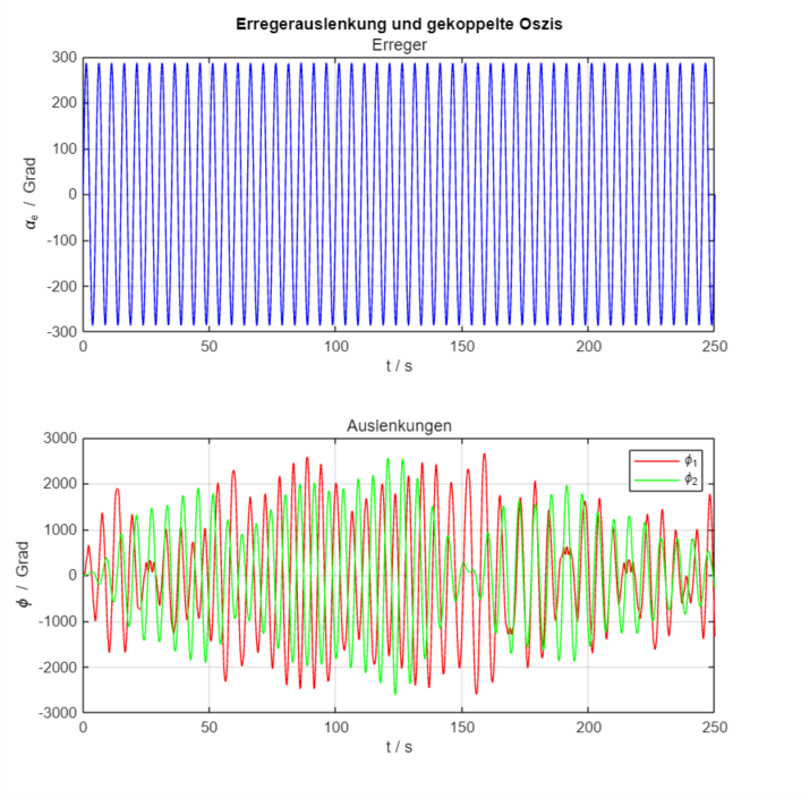
\includegraphics[height=.35\textheight]{Bilder/Kapitel-3/Chaotisches Verhalten.png}
            \caption[Chaotisches Verhalten]{Chaotisches Verhalten.}\label{Chaotisches Verhalten}
        \end{figure}

        \begin{figure}[htbp]
            \centering
            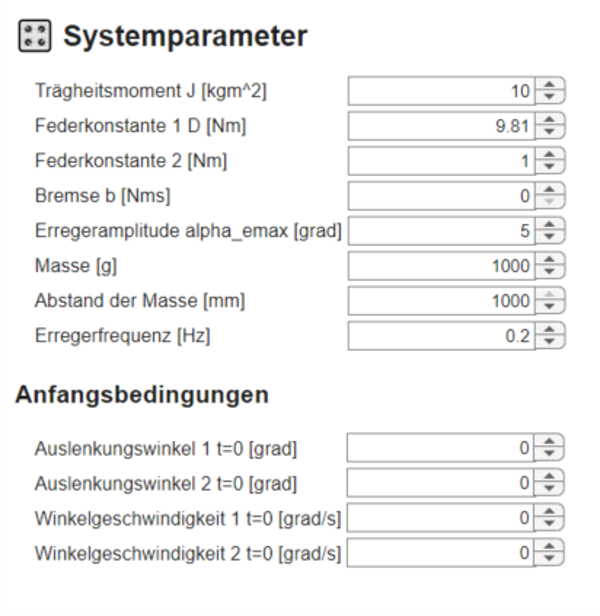
\includegraphics[height=.35\textheight]{Bilder/Kapitel-3/Systemparameter Chaotisches Verhalten.png}
            \caption[Systemparameter für chaotisches Verhalten]{Systemparameter chaotisches Verhalten.}\label{Systemparameter Chaotisches Verhalten}
        \end{figure}